\chapter{Bearing Design}

\section{Choose bearing type}
The reaction forces of bearings were calculated in Chapter 6. Since bearings selection is dependent on the ratio $ F_a/F_r $, the list below identifies the loads on each shaft:
\begin{itemize}
	\item On shaft 1, the radial loads are $ F_{1Bx} $, $ F_{1By} $, $ F_{1Dx} $, $ F_{1Dy} $; the axial load is $ F_{21z} $.
	\item On shaft 2, the radial loads are $ F_{2Ax} $, $ F_{2Ay} $, $ F_{2Dx} $, $ F_{2Dy} $; the axial load is $ F_{12z} + F_{31z} $.
	\item On shaft 3, the radial loads are $ F_{3Ax} $, $ F_{3Ay} $, $ F_{3Cx} $, $ F_{3Cy} $; the axial load is $ F_{22z} $.
\end{itemize}

Since shaft is simply supported beam (i.e. a shaft has pinned support at 1 end and roller support at the other end), the left side bearing carries both radial and axial forces while the right side bearing only carries radial force. \textbf{Table \ref{Fr/Fa}} summarizes the calculation of those loads (refer to \textbf{Table \ref{soltab}} for numerical values of the loads):

\begin{table}[ht]
	\centering
	\caption{Calculation table for limiting ratio $ F_a/F_r $}
	\begin{tabular}{lllllll}\toprule
		Sect. & $ F_x \unitp{kN} $ & $ F_y \unitp{kN} $ & $ F_z \unitp{kN} $ & $ F_r = \sqrt{F_x^2+F_y^2} \unitp{kN} $ & $ F_a = |F_z| \unitp{kN} $ & $ F_a/F_r $ \\ \midrule
		$ 1B $ & -0.56 & -0.1 & 0.22 & 0.57 & 0.22 & 0.39 \\
		$ 1D $ & -0.56 & -0.31 & 0 & 0.64 & 0 & - \\
		$ 2A $ & 1.16 & 0.07 & 0.47 & 1.16 & 0.47 & 0.41 \\
		$ 2D $ & 1.07 & -0.79 & 0 & 1.33 & 0 & - \\
		$ 3A $ & 1.76 & -0.19 & -0.69 & 1.77 & 0.69 & 0.39 \\
		$ 3C $ & -6.62 & 1.33 & 0 & 6.75 & 0 & -\\
		\bottomrule
	\end{tabular}
	\label{Fr/Fa}
\end{table}

The ratio $ F_a/F_r \geq 0.3 $ indicates the axial loads on 3 shafts are significant. Therefore, angular contact ball bearings, single row is selected. However, if the bearings are used, misalignment should not exist as recommended by the comparison table on p.72 \cite{rolling_bearings}.

The shafts are short in length, which is suitable for adjusted bearing arrangements since thermal expansion is small to axially displacing the bearings. \textbf{Figure \ref{bearing arrangement}} shows similar design and arrangement of the shafts in the speed reducer.

It is worth to mention that the actual radial load $ F_r $ and axial load $ F_a $ depend on both the bearing type and bearing arrangement. What computed in \textbf{Table \ref{Fr/Fa}} was the preliminary calculation to determine the suitable bearing type given the loads. The 'real' $ F_r $ and $ F_a $ shall be computed in the next section.

\begin{figure}[ht]
	\centering
	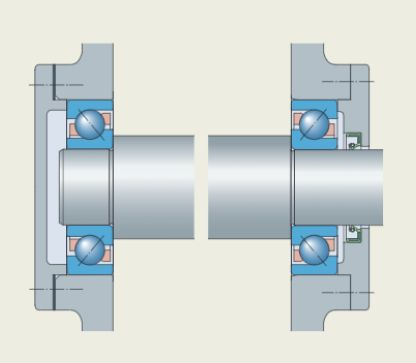
\includegraphics{bearing arrangement}
	\caption{Adjusted bearing arrangement, angular contact ball bearings arranged face-to-face. It requires proper adjustment of clearance or preload during mounting, p.76 \cite{rolling_bearings}}
	\label{bearing arrangement}
\end{figure}

Also from the previous chapter, the bore diameter $ d $ and available space $ b $ are also computed:
\[
\begin{array}{l}
d_{1B} = d_{1D} = 35 \unit{mm}, b_{O1} = 21 \unit{mm}\\
d_{2A} = d_{2D} = 45 \unit{mm}, b_{O2} = 21 \unit{mm}\\
d_{3A} = d_{3C} = 60 \unit{mm}, b_{O3} = 25 \unit{mm}\\
\end{array}
\]

From the specifications above, the bearings are selected from standard single row angular contact ball bearings product table, p.406 \cite{rolling_bearings}:
\begin{table}[ht]
	\centering
	\caption{Compact specification table of selected bearings according to SKF \cite{rolling_bearings}}
	\begin{tabular}{llll}\toprule
		Specifications & Bearings 1 & Bearings 2 & Bearings 3 \\ \midrule
		SKF designation & 7207 BE-2RZP & 7210 BE-2RZP & 7212 BEP\\
		$ d \unitp{mm} $ & 30 & 45 & 60\\
		$ D \unitp{mm} $ & 72 & 90 & 110\\
		$ B \unitp{mm} $ & 17 & 20 & 22\\
		$ C \unitp{kN} $ & 29.1 & 37.7 & 57.2\\
		$ C_0 \unitp{kN} $ & 19 & 28.5 & 45.5\\
		$ P_u \unitp{kN} $ & 0.815 & 1.22 & 1.93\\
		$ d_a \unitp{mm} $ min. & 42 & 57 & 69\\
		$ d_a \unitp{mm} $ max. & 49 & 65 & -\\
		$ D_a \unitp{mm} $ max. & 65 & 83 & 101\\
		$ r_a \unitp{mm} $ max. & 1 & 1 & 1.5\\
		$ k_r $ & 0.095 & 0.095 & 0.095\\
		\bottomrule
	\end{tabular}
	\label{bearingspecs}
\end{table}

\begin{figure}[ht]
	\centering
	\begin{subfigure}{.4\linewidth}
		\centering
		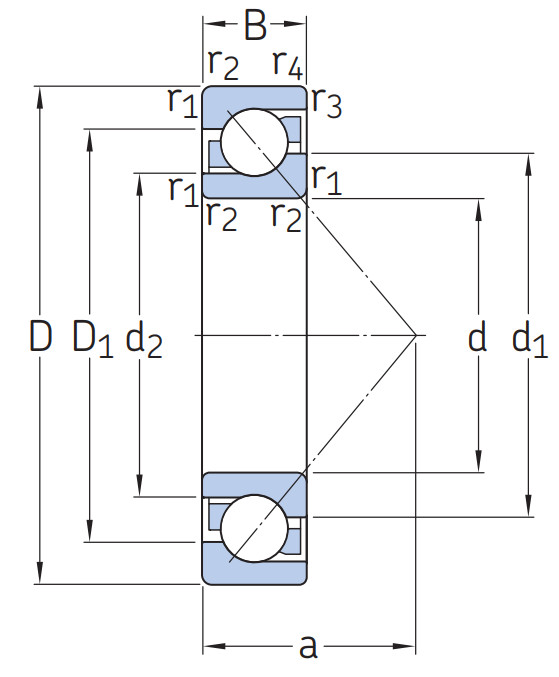
\includegraphics[width=\linewidth,keepaspectratio=true]{bearing dimension}
		\caption{Front view of single row angular contact ball bearings}
		\label{bearingdim}
	\end{subfigure}\hspace*{0.1\linewidth}
	\begin{subfigure}{.4\linewidth}
		\centering
		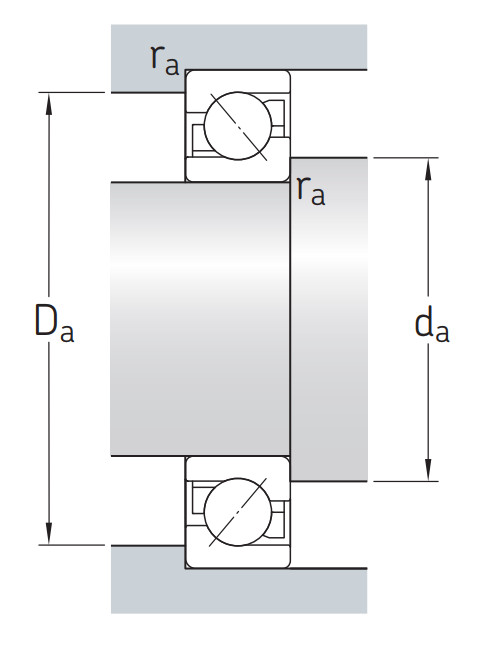
\includegraphics[width=\linewidth,keepaspectratio=true]{bearing assembly}
		\caption{Important dimensions in assembly of shaft and single row angular contact ball bearings in a housing unit}
		\label{bearingass}
	\end{subfigure}
	\caption{Important dimensions in assembly of single row angular contact ball bearings \cite{rolling_bearings}}
	\label{bearingdimass}
\end{figure}

where
\begin{itemize}
	\item $ D, B, d_a, D_a, r_a $ are the dimensions, specified in \textbf{Figure \ref{bearingdimass}}.
	\item $ C $ is the basic dynamic load rating,$ \unit{kN} $.
	\item $ C_0 $ is the basic static load rating,$ \unit{kN} $.
	\item $ P_u $ is the fatigue load limit,$ \unit{kN} $.
	\item $ A, k_r $ are the calculation factors.
\end{itemize}

Referring to \textbf{Table \ref{safety-sigma}} and \textbf{\ref{safety-tau}}, the fillet radius and shoulder diameter are in accordance with the limits provided in \textbf{Table \ref{bearingspecs}}.

\section{SKF rating life}
SKF uses a modified life factor in accordance with ISO 281 to optimize prediction of bearing life, p.89 \cite{rolling_bearings}. In terms of operating hours, the SKF rating life $ L_{nmh} $ (unit is$ \unit{h} $) is
\[L_{nmh} = \left(\dfrac{10^6}{60n}\right) a_1 a_{SKF} \left(\dfrac{C}{P}\right)^p\]
where
\begin{itemize}
	\item $ n $ is the speed of the shaft on which the bearing is mounted,$ \unit{rpm} $. The value is provided in \textbf{Table \ref{tab:my-table}}.
	\item $ a_1 $ is the life adjustment factor for reliability, Table 3, p.90 \cite{rolling_bearings}. The bearings are evaluated at $ 90\% $ reliability for common machinery. Therefore, $ a_1 = 1 $.
	\item $ a_{SKF} $ is the life modification factor, $ a_{SKF} $. The value relies on many other factors, as shown in Diagram 9, p.96 \cite{rolling_bearings}.
	
	In the diagram, the horizontal value is $ \eta_c \dfrac{P_u}{P} $, where $ \eta_c $ is the contamination factor, provided in Table 6, p.105 \cite{rolling_bearings} ($ \eta_c = 0.5 $ for normal cleanliness, chosen at worst case); $ P_u $ is the fatigue load limit, which was given in \textbf{Table \ref{bearingspecs}}; $ P $ is the equivalent dynamic bearing load, which shall be mentioned below. 
	
	The curves in the diagram correspond to a value of $ \kappa $, where $ \kappa $ is the lubrication condition (viscosity ratio) of the bearing. The value $ \kappa $ is calculated using equation on p.102 \cite{rolling_bearings}:
	\[
	\kappa = \dfrac{\nu}{\nu_1}
	\]
	where
	\begin{itemize}
		\item $ \nu $ is the actual operating viscosity of the oil or grease based oil,$ \unit{mm^2/s} $. The value depends on operating temperature, as given in Diagram 13, p.100 \cite{rolling_bearings}. Industrial machines usually operate at $ 40\degc $, however the viscosity will be considered at $ 80\degc $ in worst case. The mineral oil is ISO VG 46, which is a high quality industrial oil commonly used for mechanical lubrication. Therefore, the viscosity is $ \nu = 30 \unit{mm^2/s} $.
		\item $ \nu_1 $ is the rated viscosity, function of the mean bearing diameter and rotational speed,$ \unit{mm^2/s} $. The value is evaluated as shown in Diagram 14, p.101 \cite{rolling_bearings}. The variable in the horizontal axis is bearing mean diameter $ d_m, \unit{mm} $. It is calculated using bore diameter $ d $ and outer diameter $ D $, p.102 \cite{rolling_bearings} (all of which have been mentioned above). On the page, additional considerations are also mentioned. If the factor $ nd_m\leq 10000\unit{mm/min} $, EP (extreme pressure) and AW (anti-wear) additives are needed to reduce wear. If $ nd_m \geq 500,000\unit{mm/min} $ for $ d_m < 200 \unit{mm} $ or $ nd_m \geq 400,000 \unit{mm/min} $ for $ d_m > 200 \unit{mm} $, operating temperature must be given more attention. Since the factors in 3 shafts are outside these conditions, it is therefore omitted.
		\begin{table}[ht]
			\centering
			\caption{Calculation table for lubrication condition $ \kappa $}
			\begin{tabular}{llllllll}\toprule
				Shaft & $ d $ & $ D $ & $ d_m = 0.5(d+D) $ & $ n \unitp{rpm} $ & $ nd_m \unitp{mm/min} $ & $ \nu_1 \unitp{mm^2/s} $ & $ \kappa $ \\\midrule
				1 & 35 & 72 & 53.5 & 1455 & 77842.5 & 15 & 2.33\\
				2 & 45 & 90 & 67.5 & 514.42 & 34723.36 & 30 & 1.17\\
				3 & 60 & 110 & 90 & 181.88 & 16368.75 & 48 & 0.73\\\bottomrule
			\end{tabular}
		\end{table}
	\end{itemize}
	
	To summarize the results, \textbf{Table \ref{askf}} is provided below:
	\begin{table}[ht]
		\centering
		\caption{Calculation table life modification factor $ a_{SKF} $}
		\begin{tabular}{llllll}\toprule
			Sect. & $ P_u \unitp{kN} $ & $ P \unitp{kN} $ & $ \eta_c \dfrac{P_u}{P} $ & $ \kappa $ & $ a_{SKF} $ \\ \midrule
			$ 1B $ & 0.81 & 0.88 & 0.46 & 0.87 & 15 \\
			$ 1D $ & 0.81 & 1.08 & 0.38 & 0.87 & 10\\
			$ 2A $ & 1.22 & 1.81 & 0.34 & 0.43 & 1.1\\
			$ 2D $ & 1.22 & 2.26 & 0.27 & 0.43 & 0.9\\
			$ 3A $ & 1.93 & 2.76 & 0.35 & 0.27 & 0.22\\
			$ 3C $ & 1.93 & 7.59 & 0.13 & 0.27 & 0.2\\
			\bottomrule
		\end{tabular}
		\label{askf}
	\end{table}
	\item $ C $ is the basic dynamic load rating,$ \unit{kN} $. The value is provided in \textbf{Table \ref{bearingspecs}}.
	\item $ P $ is the equivalent dynamic bearing load,$ \unit{kN} $. It is calculated using the formula on p.398 \cite{rolling_bearings} multiplied by the gear factor 1.05 (pitch and form errors $ < 0.02 \unit{mm} $, p.93 \cite{rolling_bearings}). For the necessary factors $ X,Y,e $, Table 10 on p.400 \cite{rolling_bearings} is used for bearings pairs arranged face-to-face:
	\begin{figure}[ht]
		\centering
		\begin{subfigure}{.4\linewidth}
			\centering
			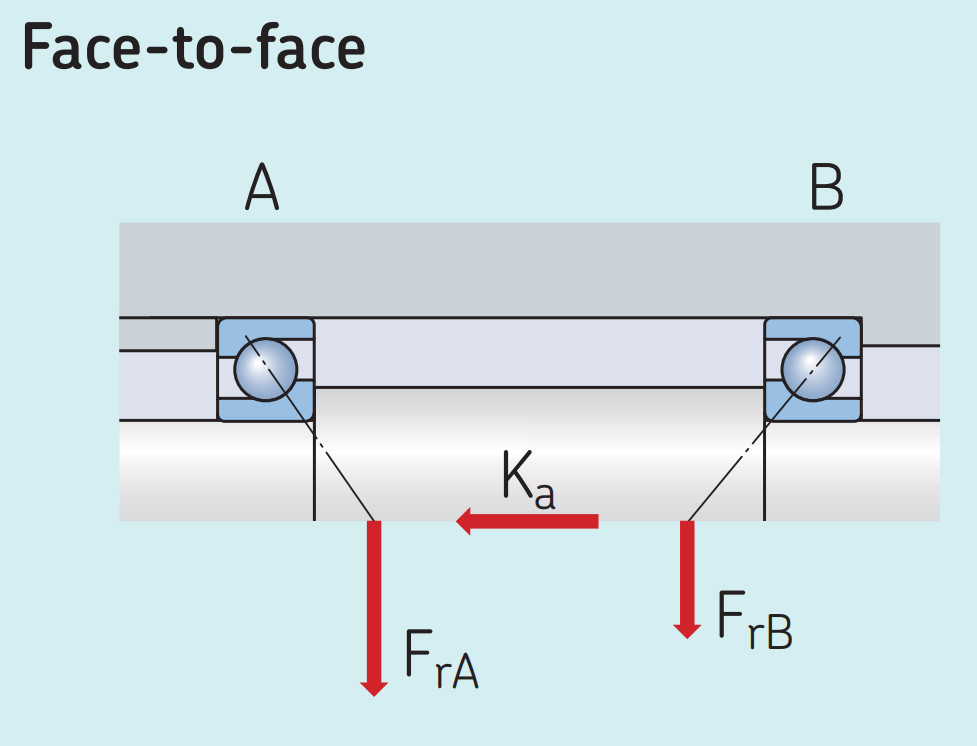
\includegraphics[width=\linewidth,keepaspectratio=true]{face2face}
			\caption{$ K_a $ points to the left}
			\label{face2face}
		\end{subfigure}\hspace*{0.1\linewidth}
		\begin{subfigure}{.4\linewidth}
			\centering
			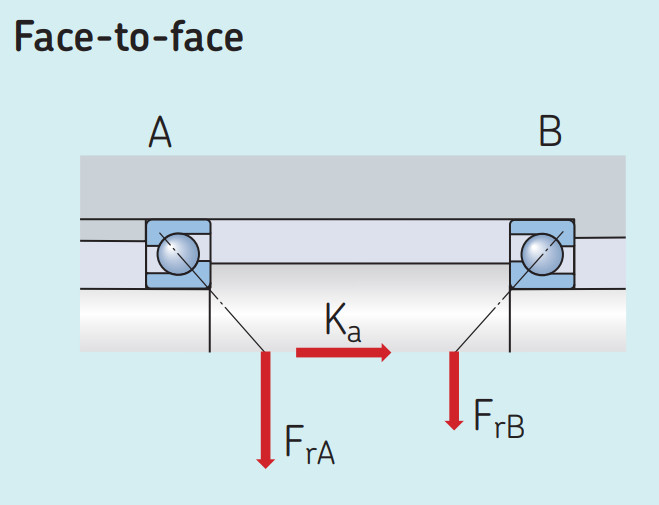
\includegraphics[width=\linewidth,keepaspectratio=true]{face2face2}
			\caption{$ K_a $ points to the right}
			\label{face2face2}
		\end{subfigure}
		\caption{Face-to-face force distribution of single row angular contact ball bearings \cite{rolling_bearings}}
	\end{figure}
	\[
	\left\{
	\begin{array}{l}
	P = 1.05(F_r + 0.55F_a), F_a/F_r \leq 1.14\\
	P = 1.05(0.57F_r + 0.93F_a), F_a/F_r > 1.14
	\end{array}
	\right.
	\]
	where
	\begin{itemize}
		\item $ F_a $ is the axial force,$ \unit{N} $. The value is computed according to Table 11, p.401 \cite{rolling_bearings}. All 3 bearings are B-series as designated on p.404 \cite{rolling_bearings}, therefore they have $ 40^\circ $ contact angle. This value corresponds to factor $ R = 0.88 $. Following the provided conditions and the direction of $ F_z $ (all units are in$ \unit{kN} $), \textbf{Table \ref{bearingforce}} is obtained:
		\begin{table}[ht]
			\centering
			\caption{Compact specification table of selected bearings according to SKF \cite{rolling_bearings}}
			\begin{tabular}{lllllll}\toprule
				Shaft & $ F_{rA} $ & $ F_{rB} $ & $ K_a = |F_z| $ & $ R(F_{rB}-F_{rA}) $ & $ F_{aA} $ & $ F_{aB} $ \\\midrule
				1 & 0.57 & 0.64 & 0.22 (\textbf{Fig. \ref{face2face}})& 0.06 (case 1b) & 0.5 & 0.72 \\
				2 & 1.16 & 1.33 & 0.47 (\textbf{Fig. \ref{face2face}})& 0.15 (case 1b) & 1.02 & 1.5 \\
				3 & 1.77 & 6.75 & 0.69 (\textbf{Fig. \ref{face2face2}})& 4.38 (case 2c) & 1.56 & 0.87 \\\bottomrule
			\end{tabular}
			\label{bearingforce}
		\end{table}
	
		where $ F_{rA} $ and $ F_{rB} $ are the radial forces of the left and right bearings, respectively.
		\item $ F_r $ is the radial force,$ \unit{kN} $. The value is provided in \textbf{Table \ref{bearingspecs}}. It is required that $ F_r $ must be larger than the minimum radial load $ F_{rm} $, which is calculated as
		\[
		F_{rm} = k_r \left(\dfrac{\nu n}{1000}\right)^{2/3}(\dfrac{d_m}{100})^2
		\]
		where
		\begin{itemize}
			\item $ k_r $ is a calculation factor, which is given in \textbf{Table \ref{bearingspecs}}.
			\item $ \nu $ is the actual operating viscosity of the oil, which was mentioned above.
			\item $ n $ is the shaft speed, which was mentioned above.
			\item $ d_m $ is the bearing mean diameter,$ \unit{mm} $. The value is computed in Table
			\begin{table}[ht]
				\centering
				\caption{Condition check for radial load for bearing pairs arranged face-to-face}
				\begin{tabular}{lllllllll}\toprule
					Shaft & $ k_r $ & $ d $ & $ D $ & $ d_m = 0.5(d+D) $ & $ F_{rA} $ & $ F_{rB} $ & $ F_{rm} $ & Condition $ F_r \geq F_{rm} $ \\\midrule
					1 & 0.095 & 35 & 72 & 53.5 & 0.57 & 0.64 & 0.34 & Satisfied \\
					2 & 0.095 & 45 & 90 & 67.5 & 1.16 & 1.33 & 0.27 & Satisfied \\
					3 & 0.095 & 60 & 110 & 90 & 1.77 & 6.75 & 0.24 & Satisfied \\\bottomrule
				\end{tabular}
				\label{Frm}
			\end{table}
		\end{itemize}
	\end{itemize}
	In total, the equivalent dynamic bearing load on each bearing is shown in \textbf{Table \ref{Pload}} (the units are in$ \unit{kN} $ except for ratio $ F_a/F_r $, which is dimensionless):
	\begin{table}[ht]
		\centering
		\caption{Calculation table for equivalent dynamic bearing load $ P $}
		\begin{tabular}{lllll}\toprule
			Sect. & $ F_r $ & $ F_a $ & $ F_a/F_r < e $ & $ P \unitp{kN} $ \\ \midrule
			$ 1B $ & 0.57 & 0.5  & 0.88<1.14 & 0.88 \\
			$ 1D $ & 0.64 & 0.72 & 1.13<1.14 & 1.08 \\
			$ 2A $ & 1.16 & 1.02 & 0.88<1.14 & 1.81 \\
			$ 2D $ & 1.33 & 1.5  & 1.12<1.14 & 2.26 \\
			$ 3A $ & 1.77 & 1.56 & 0.88<1.14 & 2.76 \\
			$ 3C $ & 6.75 & 0.87 & 0.13<1.14 & 7.59 \\
			\bottomrule
		\end{tabular}
		\label{Pload}
	\end{table}
	\item $ p $ is the exponent of the life equation. For ball bearings, $ p = 3 $.
\end{itemize}

In summary, the rating life $ L_{nmh} $ is computed in \textbf{Table \ref{ratinglife}}. According to calculation, under specified environmental conditions (normal cleanliness, working at $ 80\degc $ and $ 90\% $ reliability), the bearings are guaranteed to operate for at least $ 12,000 $ hours. This is the typical life span in machines for use 8 hours a day, but not always fully utilized, Table 1, p.88 \cite{rolling_bearings}.

SKF recommends when $ \kappa < 1 $, EP/AW additives should be used, p.102 \cite{rolling_bearings}. However, it is always possible to obtain higher lubrication condition $ \kappa $ if better viscosity oil is used (ISO VG 63). Also, the speeds of 3 shafts are not too low ($ > 10 \unitp{rpm} $) that static loading analysis is needed. Therefore, the selected SKF bearings are still valid.

The proposed bearings are listed as follows (specifications are provided in SKF bearings catalog \cite{rolling_bearings}):
\begin{itemize}
	\item Shaft 1: 7207 BE-2RZP
	\item Shaft 2: 7210 BE-2RZP
	\item Shaft 3: 7212 BEP
\end{itemize}
\begin{table}[ht]
	\centering
	\caption{Calculation table for SKF rating life $ L_{nmh} $ in hours}
	\begin{tabular}{llllll}\toprule
		Sect. & $ n \unitp{rpm} $ & $ a_{SKF} $ & $ C \unitp{kN} $ & $ P \unitp{kN} $ & $ L_{nmh} \unitp{h} $ \\ \midrule
		$ 1B $ & 1455   & 15   & 29.1 & 0.88 & $ 6,201,499.81 $ \\
		$ 1D $ & 1455   & 10   & 29.1 & 1.08 & $ 2,238,026.65 $ \\
		$ 2A $ & 514.42 & 1.1  & 	37.7 & 1.81 & $ 321,910.25 $ \\
		$ 2D $ & 514.42 & 0.9  & 37.7 & 2.26 & $ 135,097.87 $ \\
		$ 3A $ & 181.88 & 0.22 & 66.3 & 2.76 & $ 278,897.56 $ \\
		$ 3C $ & 181.88 & 0.2  & 66.3 & 7.59 & $ 12,211.88 $ \\
		\bottomrule
	\end{tabular}
	\label{ratinglife}
\end{table}